%% Encoding: ISO8859-1 %%

\section{Allgemeines}
\frame{
\frametitle{Allgemeines}
\begin{itemize}
    \item neue Art von Schaltkreis (Nanoelektronik) 
    \item Signale als Token auf Kabeln 
    \item Fluktuation der Token als treibende Kraft f�r Berechnungen
\end{itemize}
}
\section{Polare Token-pass Schaltkreise}
\frame{
\frametitle{Polare T-Elemente}
\begin{columns}[T]
\begin{column}[T]{5cm}
    \begin{itemize}
        \item Pfeile geben Richtung vor
        \item Tokens werden nur in dieser vearbeitet
    \end{itemize}
\end{column}
    \begin{column}[T]{5cm}
        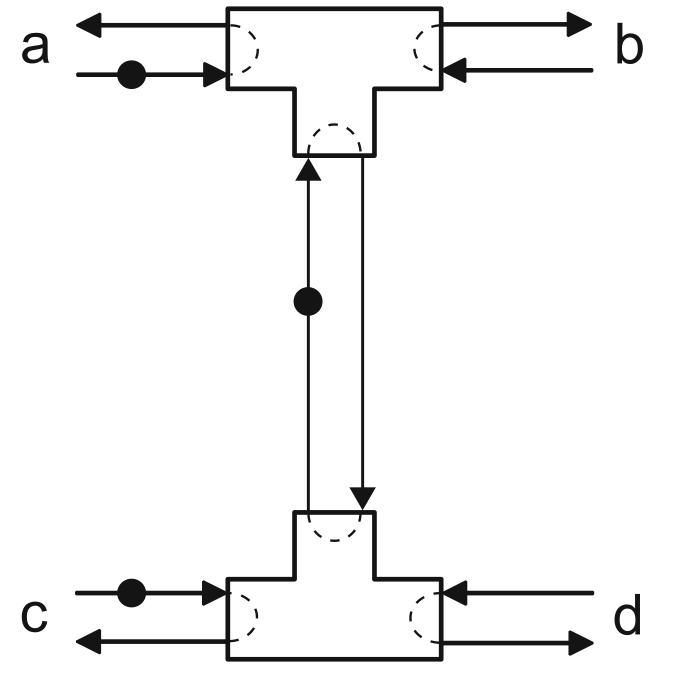
\includegraphics[height=5cm]{bilder/polarElemente.png} 
    \end{column}
\end{columns}
}
\section{Nicht-polare Token-pass Schaltkreise}
\frame{
\frametitle{Nicht-polare T-Elemente}
\begin{columns}[T]
\begin{column}[T]{5cm}
    \begin{itemize}
        \item Tokens k�nnen beide Richtungen nehmen
        \item Kreise bzw. Blanksymbole geben Einschr�nkung
    \end{itemize}
\end{column}
    \begin{column}[T]{5cm}
        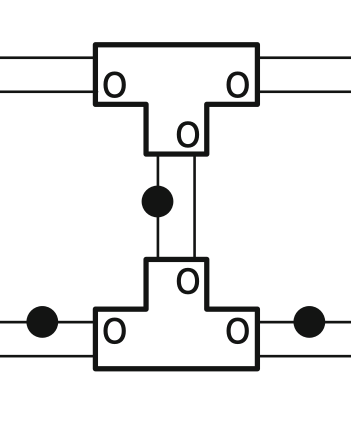
\includegraphics[height=5cm]{bilder/nonPolarElemente.png} 
    \end{column}
\end{columns}
}

